% documentation on tikz-uml:
% http://www.ensta-paristech.fr/~kielbasi/tikzuml/index.php?lang=en&id=doc#t-1.1
\begin{tikzpicture}

\umlclass{Protein}{
  concentration \\
  $K_m$ \\
  $n$ \\
}{}
\umlclass[y=-6]{BioBrick}{
  proteins \\
  gates \\
}{}
\umlclass[x=6,y=-6]{Circuit}{bricks[]}{}

\umlclass[x=6,y=0]{SBML}{circuit}{}



\umlassoc[mult1=*, mult2=*]{Protein}{BioBrick}
\umlassoc[mult1=*, mult2=*]{Circuit}{BioBrick}
\umlinherit[geometry=-|, arg1=represents,align1=right]{SBML}{Circuit}
\end{tikzpicture}

